\secrel{\vim}\label{vim}\secdown


\includegraphics[height=0.5\textheight]{logo/vim.png}

\secrel{Установка под \win}

\menu{\winr cmd > \url{http://www.vim.org/} > Download > PC: MS-DOS and
MS-Windows > \href{ftp://ftp.vim.org/pub/vim/pc/gvim74.exe}{\file{gvim74.exe}}}

\menu{Vim 7.4 Setup>This will install>Да}

\menu{License>I'm Angry}

\menu{Installation Options>\checkbox\ Create .bat files>Next}

\menu{Installation Folder>Install}

\menu{Completed>Close}

\menu{Do you want to see README>\textbf{Да}}
\bigskip

Теперь можно настроить темную тему и выключение подстветки синтаксиса, по
умолчанию после установки используется светлая тема и подстветка выключена:

\nopagebreak
\menu{меню>Правка>Настройка запуска}
\bigskip

Переходим в конец файла и включаем \emph{режим вставки}

\keys{Ctrl+Down}\ \keys{Ins}\ \keys{Enter}\keys{Enter}

\begin{lstlisting}
syntax on
colorscheme pablo
\end{lstlisting}
\bigskip

Выходим в \emph{режим команд} и принудительно сохраняем

\keys{Esc}:\keys{w}\keys{!}\keys{Enter}\keys{Enter}
\bigskip

\textbf{Выходим из \vim}

\keys{Esc}:\keys{q}\keys{!}\keys{Enter}

\bigskip
Если не получилось (под Windows 7):

\bigskip
\menu{\winr cmd > \file{/Program Files (x86)/Vim/}}
\bigskip

Копируем файл \file{\_vimrc}\ в любой каталог, например в \file{/tmp/},
затем \menu{\rms\rms>Edit with Vim}, и повторяем редактирование еще раз.

\bigskip
Затем копируем \file{\_vimrc}\ обратно в \file{/Program Files (x86)/Vim/}\ с
заменой.

\bigskip
Если теперь открыть на редактирование тот же файл, или любой другой текстовый,
получим более удобный вид: для файлов известных типов будет работать подсветка
синтаксиса.

\nopagebreak\bigskip
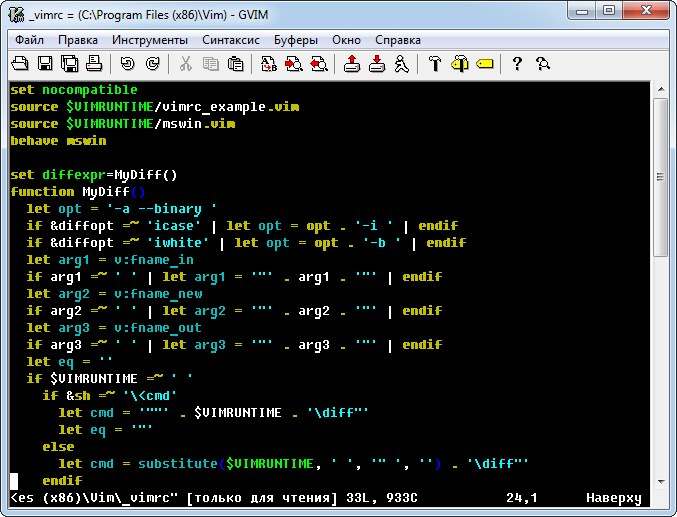
\includegraphics[height=0.7\textheight]{ide/vim28.png}

\secrel{Выход из \vim}

\keys{Esc}\ :\ \keys{!}\ \keys{q}\ \keys{Enter}

\secrel{Выход с автосохранением}

\keys{Esc}\ \keys{Shift+Z}\ \keys{Shift+Z}

\secrel{Переход в режим редактирования}

\vim\ запускается в \emph{командном режиме}, для перехода в режим редактирования
используются следующие клавиатурные команды:

\begin{itemize}
  \item \keys{Ins}\ или \keys{i}: включение \emph{режима вставки} по текущему
  положению курсора
  \item \keys{Ins}\keys{Ins}\ или \keys{r}: включение \emph{режима перезаписи}
  поверх текста после курсора
  \item \keys{Shift+A}: включение режима вставки \emph{в конец текущей строки}
\end{itemize}

\secrel{Переход в режим команд}

\keys{Esc}

\secrel{Запись редактируемого файла}

\keys{Esc}\ :\ \keys{w}\ \keys{Enter}
\bigskip

Если выводится предупреждение типа ``файл защищен от записи'' или подобное,
может сработать принудительная запись:

\bigskip
\keys{Esc}\ :\ \keys{!}\ \keys{w}\ \keys{Enter}

\secrel{Перезагрузка файла}

Для перезагрузки возможно изменененного извне файла или отмены всех
несохраненных изменений

\bigskip
\keys{Esc}\ :\ \keys{e}\ \keys{Enter}

\secrel{Отмена последних изменений (undo)}

\keys{Esc}\keys{u}\keys{u}\ldots

\secup

